\section{Reto de extensión}

Se implementó el reto de extensión propuesto por el instructivo: convertir el procedimiento \texttt{saludo} en un servicio multi-operación \texttt{calc.cgi}, expuesto en \texttt{/rpc/calc.cgi}, que resuelve las cuatro operaciones aritméticas básicas usando \texttt{bash} y \texttt{bc}, y que implementa un esquema mínimo de claves de idempotencia mediante la cabecera \texttt{Idempotency-Key}, almacenando las respuestas previas en \texttt{/var/tmp/rpc-cache}.

\subsection*{Invocación de las operaciones}
\begin{lstlisting}[language=bash]
$ curl -s 'http://localhost:8080/rpc/calc.cgi?op=sum&a=3&b=4'
{"servicio":"calc","op":"sum","a":3,"b":4,"resultado":7}

$ curl -s 'http://localhost:8080/rpc/calc.cgi?op=div&a=5&b=0'
{"error":"división entre cero"}
\end{lstlisting}

La división entre cero devuelve el código de estado \texttt{422 Unprocessable Entity}, verificado con \texttt{curl -sD -}, en vez de un error genérico:

\begin{lstlisting}
HTTP/1.1 422 Unprocessable Entity
Content-Type: application/json; charset=UTF-8
\end{lstlisting}

\subsection*{Verificación de idempotencia}

Se realizaron dos peticiones consecutivas con la misma cabecera \texttt{Idempotency-Key}, pero con operandos distintos en la segunda, para comprobar que el servicio responde con el resultado cacheado de la primera invocación en lugar de recalcular:

\begin{lstlisting}[language=bash]
$ curl -s -H 'Idempotency-Key: abc123' \
    'http://localhost:8080/rpc/calc.cgi?op=mul&a=6&b=7'
{"servicio":"calc","op":"mul","a":6,"b":7,"resultado":42}

$ curl -s -H 'Idempotency-Key: abc123' \
    'http://localhost:8080/rpc/calc.cgi?op=mul&a=999&b=999'
{"servicio":"calc","op":"mul","a":6,"b":7,"resultado":42}
\end{lstlisting}

\begin{figure}[H]
\centering
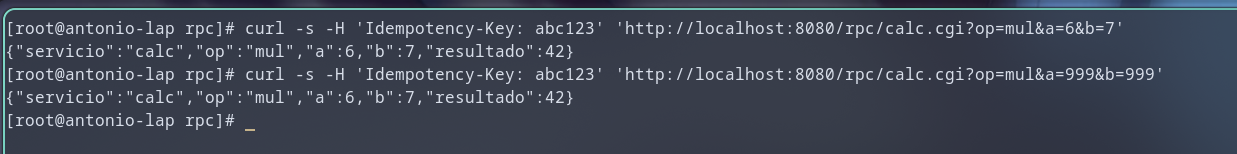
\includegraphics[width=\linewidth]{../src/ss/2.6.png}
\caption{Verificación de idempotencia: dos invocaciones con la misma clave \texttt{abc123} devuelven el resultado de la primera.}
\label{fig:p1-idempotencia}
\end{figure}

La Figura~\ref{fig:p1-idempotencia} muestra el comportamiento clave del mecanismo: la segunda invocación pide \texttt{a=999\&b=999}, pero la respuesta repite \texttt{a:6, b:7, resultado:42} —el contenido cacheado en \texttt{/var/tmp/rpc-cache/abc123} durante la primera llamada. El servidor ni siquiera evalúa la operación: al encontrar un archivo con el nombre de la clave, lo devuelve y termina. Esto materializa la técnica descrita en el marco teórico para aproximar la semántica \emph{exactly-once}: el cliente puede reintentar libremente (comportamiento \emph{at-least-once}) porque el filtrado de duplicados del servidor (comportamiento \emph{at-most-once}) garantiza que el efecto se produzca una sola vez. La combinación de ambos es precisamente lo que un reintento con \emph{backoff} necesita para ser seguro sobre operaciones no idempotentes.
